\section{Performance Evaluation and Comparison}\raggedbottom

\subsection{Quality}
To evaluate the clustering performed by SUBCLU and FIRES, we implemented some of the evaluation measures presented in the paper \citep{10.1145/2063576.2063774}. All these external evaluation measures work on comparing a resulting clustering to a known ground truth.

First, the F1-measure, which evaluates how good and precisely the true clusters are represented by the found clusters. A good representation is achieved when all true clusters are found and each found cluster $c_{found}$ has as many points as possible in common with a true cluster $c_{true}$ and as few incorrectly assigned points as possible. To cover both these aspects of a cluster representation, the F1-measure employs two other external performance metrics called recall and precision:
\begin{equation}
recall(c_{found},c_{true}) = \frac{TP}{TP + FN} = \frac{|c_{found} \cap c_{true}|}{|c_{true}|}.
\end{equation}

\begin{equation}
precision(c_{found},c_{true}) = \frac{TP}{TP + FP} = \frac{|c_{found} \cap c_{true}|}{|c_{found}|}.
\end{equation}

and computes the harmonic mean of them as follows:
\begin{equation}
F1(c_{found},c_{true}) = \frac{2\cdot recall(c_{found},c_{true})\cdot precision(c_{found},c_{true})}{recall(c_{found},c_{true}) + precision(c_{found},c_{true})}.
\end{equation}

The overall F1-measure of two clusterings $C_{found}$ and $C_{true}$ is then the mean of all maximum F1-measures of all clusters. We can differentiate between three computations of the overall F1-measure, depending on which clusters we are considering. If we are iterating over the true clusters, then we call it F1-Recall:
\begin{equation}
F1^{R}(C_{true},C_{found}) = \frac{1}{|C_{true}|} \sum _{c_{i}\in C_{true}} \max _{c_{j}\in C_{found}} \{F1(c_{i},c_{j})\}.
\end{equation}

Which can be seen as the recall but at the clustering level. As we can see, we are only considering found clusters that maximize the formula. Therefore, all redundant subspace clusters that are found in lower-dimensional projections and produced by a subspace clustering algorithm are not affecting the clustering quality negatively as they should do. On the other hand, iterating over found clusters yields the F1-Precision:
\begin{equation}
F1^{P}(C_{found},C_{true}) = \frac{1}{|C_{found}|} \sum _{c_{i}\in C_{found}} \max _{c_{j}\in C_{true}} \{F1(c_{i},c_{j})\}.
\end{equation}

Which is like precision but at the clustering level. Contrary to F1-Recall, F1-Precision is redundancy-aware, but since we are skipping true subspace clusters that are not a perfect match of found clusters with respect to the F1-measure, F1-Precision is not identification-aware because missing true clusters are not covered and are not affecting the quality.

A third form of the overall F1-measure can be computed by the mean of the F1-measures of true clusters and merged sets of found clusters. This measure is called F1-Merge and defined as follows:
\begin{equation}
\begin{multlined}
F1^{M}(C_{found},C_{true}) = \frac{1}{|C_{true}|} \sum _{c_{i}\in C_{true}} F1(c_{i},\acute{c}), \textrm{where}\\
\acute{c} = \bigcup _{c_{j}\in C_{found}} \Biggl\{c_{j} \mid \frac{|c_{j} \cap c_{i}|}{|c_{i}|} \geq \frac{|c_{j} \cap c_{t}|}{|c_{t}|} \forall  c_{t} \in C_{true} \Biggl\}.
\end{multlined}
\end{equation}

So, for each true cluster we merge all found clusters that share their best matching true clusters. Since we are iterating over true clusters, the F1-Merge measure is identification-aware but it is not redundancy-aware because found clusters in lower-dimensional projections are merged together with their higher-dimensional subspace clusters. In addition, merging found clusters together does not penalize split found clusters that represent one true cluster.

All three forms of the F1-measure are adapted from variants used to evaluate classification tasks and are not developed to evaluate subspace clustering. They are object-based because they work on comparing clusters of two clusterings based on data objects within the clusters. However, they are not subspace-aware since they are computed without regard to information about the subspaces in which the clusters exist. So, finding a true cluster in a different subspace than the true desired one will not affect the quality score. Therefore, high quality scores need not necessarily mean good subspace clustering. 

Subspace-aware quality measures are more adequate to the problem since we do not just want to check if true clusters are found but also if they are detected in the right subspaces.

The key idea that enables subspace-aware evaluations is to consider every data object as a set of different subobjects(also called micro-objects) rather than  one object in full-dimensional feature space. So, in a dataset with n objects and d dimensions, there will be n$\times$d micro-objects. A subspace cluster is then represented as a subset of these micro-objects. For example, let $c = \{1, 2, 3\}$ be a cluster in subspace $\{c,e,f\}$, then we redefine $c$ as $c = \{o_{i,j} | i\in \{1,2,3\} \wedge j\in \{c,e,f\}\} =  \{o_{1c},o_{2c},o_{3c},o_{1e},o_{2e},o_{3e},o_{1f},o_{2f},o_{3f}\}$. As a result, we now have the subspace information. 
\begin{center}
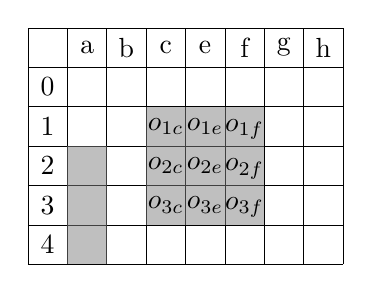
\begin{tikzpicture}[thick,fill opacity=0.5]
\draw[step=0.5cm,black,very thin] (-1.5,-1) grid (2.5,2);
\node at (-0.75,+1.75) [text opacity=1] {a};
\node at (-0.25,+1.75) [text opacity=1]{b};
\node at (+0.25,+1.75) [text opacity=1]{c};
\node at (+0.75,+1.75) [text opacity=1]{e};
\node at (+1.25,+1.75) [text opacity=1]{f};
\node at (+1.75,+1.75) [text opacity=1]{g};
\node at (+2.25,+1.75) [text opacity=1]{h};
\node at (-1.25,+1.25) [text opacity=1]{0};
\node at (-1.25,+0.75) [text opacity=1]{1};
\node at (-1.25,+0.25) [text opacity=1]{2};
\node at (-1.25,-0.25) [text opacity=1]{3};
\node at (-1.25,-0.75) [text opacity=1]{4};
\fill[gray] (-1,-1) rectangle (-0.5,-0.5);
\fill[gray] (-1,-0.5) rectangle (-0.5,0);
\fill[gray] (-1,0) rectangle (-0.5,0.5);
\fill[gray] (+0,0) rectangle (0.5,0.5);
\fill[gray] (+0.5,1) rectangle (1,0.5);
\fill[gray] (+0.5,0) rectangle (1,0.5);
\fill[gray] (+1,0) rectangle (1.5,0.5);
\fill[gray] (+1,0.5) rectangle (1.5,1);
\fill[gray] (0,0.5) rectangle (0.5,1);
\fill[gray] (+0,-0.5) rectangle (0.5,0);
\fill[gray] (+0.5,-0.5) rectangle (1,0);
\fill[gray] (+1,-0.5) rectangle (1.5,0);
\node at (+0.25,+0.75) [text opacity=1]{$o_{1c}$};
\node at (+0.25,+0.25) [text opacity=1]{$o_{2c}$};
\node at (+0.25,-0.25) [text opacity=1]{$o_{3c}$};
\node at (+0.75,+0.75) [text opacity=1]{$o_{1e}$};
\node at (+0.75,+0.25) [text opacity=1]{$o_{2e}$};
\node at (+0.75,-0.25) [text opacity=1]{$o_{3e}$};
\node at (+1.25,+0.71) [text opacity=1]{$o_{1f}$};
\node at (+1.25,+0.21) [text opacity=1]{$o_{2f}$};
\node at (+1.25,-0.28) [text opacity=1]{$o_{3f}$};
\end{tikzpicture}
\end{center}

The first subspace-aware evaluation measure we are going to look at is called RNIA (relative non-intersecting area). RNIA considers two clustering as finite sets of micro-objects and measures their similarity as follows:
\begin{equation} \label{eq:8}
RNIA(C_{found},C_{true}) = \frac{|U| - |I|}{|U|}.
\end{equation}

Where $U$ denotes the union of micro-objects of both clusterings and $I$ the intersection of their micro-objects. A good similarity is reached by a high hit rate and a low false positive rate of micro-objects. But this formula needs to be adjusted to cover micro-objects that belong to more than one subspace cluster due to simultaneously overlapping clusters and subspaces. A solution that redefines $U$ and $I$ was introduced in \citep{10.1109/TKDE.2006.106}, where $U = \sum_{i,j} \max(count_{true}(o_{i,j}), count_{found}(o_{i,j}))$ and $I = \sum_{i,j} \min(count_{true}(o_{i,j}), count_{found}(o_{i,j}))$ and $count$ the number of appearance in different subspace clusters. Briefly explained, each micro-object that is shared by different clusters will be dissolved and treated as several new unique micro-objects that share the same position in the matrix.

The best result is $RNIA = 0$ when both clusterings are equal $U = I$ and the worst result is $RNIA = 1$ when there is no intersection at all between true and found micro-objects.

Since the RNIA measure works at micro-object level and not on cluster level, neither clusters that include more than one class label nor splits and merges of found clusters are penalized.

To keep it simple for readers and similar to other quality scores, we compute $1 - RNIA$ so that 0 is the worst quality and 1 is the best.

Another subspace-aware evaluation measure is called CE (clustering error). CE functions similar to RNIA but it overcomes the inability of RNIA to detect splits and merges of found clusters by taking cluster-coverage into account. So, Instead of comparing true micro-objects with found micro-objects all at once without regard to which subspace clusters the micro-objects belong, CE searches for each true subspace cluster its best matching found cluster that has the most intersection of micro-objects with it and for each found subspace cluster its best matching true cluster. No true cluster is assigned to more than one found cluster and vice versa. This assignment should be chosen in such a way that it maximizes $D_{max}$ the sum over the intersections of each selected pair. The overall CE measure is then defined as follows:
\begin{equation} \label{eq:9}
CE(C_{found},C_{true}) = \frac{|U| - D_{max}}{|U|}.
\end{equation}

One way to find the perfect 1:1 assignment of clusters in relation to micro-objects intersection is to compute a square matrix of shape $max(|C_{found}|,|C_{true}|) \times max(|C_{found}|,|C_{true}|$) where 
an element represents the cardinality of the micro-objects' intersection of one true cluster and one found cluster. In case $|C_{found}| \neq |C_{true}|$ additional rows or columns are filled with zeros. Now, after computing the matching matrix, calculating $D_{max}$ would be like solving a maximum weight matching problem.

The best score $CE = 0$, is achieved when $|C_{found}| = |C_{true}|$ and for each true cluster there is a found cluster with the same micro-objects and vice versa. $U$ is computed as for RNIA and $D_{max}$ is not affected by overlapped subspaces and clusters.

As for the RNIA measure, we compute $1 - CE$ so that 0 is the worst quality and 1 is the best.

The last evaluation measure, called E4SC, was introduced for the first time in \citep{10.1145/2063576.2063774}. This novel quality measure has all the characteristics that a good subspace evaluation measure should have. It fulfills the subspace-awareness and the object-awareness criteria by using a subspace-aware version of the F1-measure in which recall and precision are redefined as follows:
\begin{equation}
recall_{sc}(c_{found},c_{true}) = \frac{|microObjects(c_{found}) \cap microObjects(c_{true})|}{|microObjects(c_{true})|}.
\end{equation}

\begin{equation}
precision_{sc}(c_{found},c_{true}) = \frac{|microObjects(c_{found}) \cap microObjects(c_{true})|}{|microObjects(c_{found})|}.
\end{equation}

And their harmonic mean:
\begin{equation}
F1_{sc}(c_{found},c_{true}) = \frac{2\cdot recall_{sc}(c_{found},c_{true})\cdot precision_{sc}(c_{found},c_{true})}{recall_{sc}(c_{found},c_{true}) + precision_{sc}(c_{found},c_{true})}.
\end{equation}

As for the non-subspace-aware overall F1-measure of two clusterings, we have $F1^{R}_{sc}$:

\begin{equation}
F1^{R}_{sc}(C_{true},C_{found}) = \frac{1}{|C_{true}|} \sum _{c_{i}\in C_{true}} \max _{c_{j}\in C_{found}} \{F1_{sc}(c_{i},c_{j})\}.
\end{equation}

And $F1^{P}_{sc}$:
\begin{equation}
F1^{P}_{sc}(C_{found},C_{true}) = \frac{1}{|C_{found}|} \sum _{c_{i}\in C_{found}} \max _{c_{j}\in C_{true}} \{F1_{sc}(c_{i},c_{j})\}.
\end{equation}
Which evaluates the representation of the true clusters.  

The symmetric evaluation measure E4SC is then defined as the harmonic mean of $F1^{R}_{sc}$ and $F1^{P}_{sc}$:
\begin{equation}
E4SC(C_{found},C_{true}) = \frac{2\cdot F1^{R}_{sc}(C_{true},C_{found})\cdot F1^{P}_{sc}(C_{found},C_{true})}{F1^{R}_{sc}(C_{true},C_{found}) + F1^{P}_{sc}(C_{found},C_{true})}.
\end{equation}

Missing true subspace clusters and redundant found clusters are detected and penalized by $F1^{R}_{sc}$ and $F1^{P}_{sc}$ respectively. 

We applied SUBCLU and FIRES with DBSCAN as a clustering method to both synthetic and real world datasets. But since we do not have any information about the true subspace clusters within the real world datasets, we adjust $C_{true}$ to represent the partitioning of the data objects in the full space, which is known due to provided class labels of all objects.

Three real world datasets were clustered and evaluated. First, a vowel dataset that contains information about sounds of the eleven steady state vowels of English spoken by multiple speakers. Second, a diabetes dataset which contains diagnostic measurements of diabetic and non-diabetic persons. Last, a glass dataset that contains examples of the chemical analysis of 7 different types of glass. All real world datasets are from the UCI machine learning repository \citep{Dua:2019}. In addition, we evaluated the clustering resulting from applying SUBCLU and FIRES to the synthetic datasets D05 and D10.

The best quality scores achieved for each dataset can be seen in Table~\ref{tab:quality} below:

\begin{table}[H]
\centering
\begin{tabular}{|c|c|c|c|c|c|c|c|}
	\hline
	&&\small F1-Recall&\small F1-Precision&\small F1-Merge&\small RNIA&\small CE&\small E4SC\\
	\hline
	\hline
	\multirow{2}{3.8em}{$\underset{528\times10}{\textrm{Vowel}}$}&\small SUBCLU&0.52&0.24&0.17&0&0&0.24\\
	&\small FIRES&0.28&0.24&0.17&0.52&0.10&0.13\\
	\hline
	\hline
	\multirow{2}{3.8em}{$\underset{768\times8}{\textrm{Diabetes}}$}&\small SUBCLU&0.65&0.55&0.65&0.01&0.01&0.46\\
	&\small FIRES&0.64&0.14&0.66&0.16&0.13&0.11\\
	\hline
	\hline
	\multirow{2}{3.8em}{$\underset{214\times9}{\textrm{Glass}}$}&\small SUBCLU&0.58&0.51&0.27&0&0&0.45\\
	&\small FIRES&0.40&0.55&0.27&0.54&0.23&0.23\\
	\hline
	\hline
	\multirow{2}{3.8em}{$\underset{1595\times5}{\textrm{D05}}$}&\small SUBCLU&0.99&0.84&0.20&0.15&0.15&0.78\\
	&\small FIRES&0.81&0.28&0.78&0.27&0.18&0.26\\
	\hline
	\hline
	\multirow{2}{3.8em}{$\underset{1595\times10}{\textrm{D10}}$}&\small SUBCLU&1&0.84&0.20&0.01&0.01&0.71\\
	&\small FIRES&0.91&0.34&0.68&0.12&0.10&0.29\\
	\hline
\end{tabular}
\caption{Quality comparison of SUBCLU and FIRES.}
\label{tab:quality}
\end{table}

\begin{table}[H]
	\centering
	\begin{tabular}{|c|c|c|c|c|c|}
		\hline
		&&\small F1-Merge&\small RNIA&\small CE&\small E4SC\\
		\hline
		\hline
		\multirow{2}{3.8em}{$\underset{990\times10}{\textrm{Vowel}}$}&\small SUBCLU&0.24&0.39&0.04&0.03\\
		&\small FIRES&0.16&0.14&0.02&0.03\\
		\hline
		\hline
		\multirow{2}{3.8em}{$\underset{768\times8}{\textrm{Diabetes}}$}&\small SUBCLU&0.74&0.01&0.01&0.46\\
		&\small FIRES&0.52&0.27&0.12&0.1\\
		\hline
		\hline
		\multirow{2}{3.8em}{$\underset{214\times9}{\textrm{Glass}}$}&\small SUBCLU&0.50&0.01&0.00&0.38\\
		&\small FIRES&0.30&0.45&0.21&0.24\\
		\hline
	\end{tabular}
	\caption{Quality comparison of SUBCLU and FIRES from \citep{10.1145/2063576.2063774}.}
	\label{tab:scoresFromPaper}
\end{table}

The evaluation scores regarding the Vowel dataset look noticeably dissimilar because the dataset has been updated and does not exist in the same shape as back then. Otherwise, the results look similar, taking into consideration that we do not know whether the authors did preprocess the datasets before clustering or not. We did not cluster the other real world datasets from the paper because we plotted them and did not find any clusters that could be detected.

To notice here is that SUBCLU has very low RNIA and CE scores. This can be explained by the huge number of redundant clusters produced by SUBCLU, which makes the cardinality of the union of micro-objects too high compared to the intersection  $|U| - |I| \approx |U|$ in Equation \ref{eq:8} and to $D_{max}$ in Equation \ref{eq:9} $|U| - D_{max} \approx |U|$. However, this redundancy leads to good cluster coverage, the reason why SUBCLU achieves good F1 scores. 

\subsection{Scalability}
Besides producing results of high quality, algorithms should also perform efficiently. Since we are dealing with high-dimensional data, it is expected for subspace clustering algorithms to perform slower when increasing the data dimensionality or the number of data objects, but also other factors like increasing the number of subspace clusters or their dimensionalities would affect the runtime of a subspace clustering algorithm.

For the following experiments, we chose DBSCAN as a clustering method for FIRES and we measured the runtime of all steps. 

First, to test the behavior with respect to increasing the dimensionality of the dataset, we applied both algorithms to six datasets having 5, 10, 15, 20, 25, 50 dimensions respectively. Each dataset consists of about 1600 points and 10 subspace clusters. The dimensionalities of the subspace clusters increase with increasing the dimensionality of the dataset. The results can be seen in Figure~\ref{fig:cluster_xd_xn_10sc}. In addition, to see the impact of the number of subspace clusters on the runtime of both algorithms, we redid the experiment on six other datasets with the same data dimensionalities but with only 1 subspace cluster per dataset. The results are illustrated in Figure~\ref{fig:cluster_xd_1000n_1sc} below:
\begin{figure}[H]
	\centering
	\begin{minipage}{0.5\textwidth}
		\centering
		\includegraphics[width=0.9\textwidth]{bilder/cluster_xd_xn_10sc}
		\caption{10 subspace clusters per dataset.}
		\label{fig:cluster_xd_xn_10sc}
	\end{minipage}\hfill
	\begin{minipage}{0.5\textwidth}
		\centering
		\includegraphics[width=0.9\textwidth]{bilder/cluster_xd_1000n_1sc}
		\caption{1 subspace clusters per dataset.}
		\label{fig:cluster_xd_1000n_1sc}
	\end{minipage}
\end{figure}
As we can see in Figure~\ref{fig:cluster_xd_xn_10sc} SUBCLU scales exponentially with respect to the data dimensionality and needed about an hour to cluster the dataset with 20 dimensions, the reason why we did not apply it to the other datasets with more dimensions. All studies like \citep{10.14778/1687627.1687770} and \citep{10.1145/2063576.2063774} that include SUBCLU have also noticed such inefficient performance. This is caused by the bottom-up heuristic used by SUBCLU to investigate possible subspaces. It is not clear how FIRES exactly scales because the number of runtime measurements is not enough and SUBCLU has too high runtimes compared to FIRES. However, it is noticeably faster, because it jumps from the 1-dimensional base-clusters directly to subspace clusters of maximal dimensionalities without going through the whole space of all possible subspaces.

The runtime drops significantly if there are fewer subspace clusters as shown in Figure~\ref{fig:cluster_xd_1000n_1sc}, but even with only one subspace cluster, SUBCLU still scales at least quadratic. 

To measure the time complexities of SUBCLU and FIRES with respect to the number of points in the dataset, we applied both on five datasets having between 1500--5500 data points, Figure~\ref{fig:cluster_10d_xn_10sc}. Each data set consists of 10 dimensions and 10 subspace clusters. Additionally, we redid the experiment with only 2 subspace cluster per dataset. The results are in Figure~\ref{fig:cluster_10d_xn_2sc}.
\begin{figure}[H]
	\centering
	\begin{minipage}{0.5\textwidth}
		\centering
		\includegraphics[width=0.9\textwidth]{bilder/cluster_10d_xn_10sc}
		\caption{10 subspace clusters per dataset.}
		\label{fig:cluster_10d_xn_10sc}
	\end{minipage}\hfill
	\begin{minipage}{0.5\textwidth}
		\centering
		\includegraphics[width=0.9\textwidth]{bilder/cluster_10d_xn_2sc}
		\caption{2 subspace clusters per dataset.}
		\label{fig:cluster_10d_xn_2sc}
	\end{minipage}
\end{figure}
Increasing the number of data points in the dataset does not affect the runtime as much as the data dimensionality. However, if this number is combined with a certain dimensionality, then it could lead to a very high runtime of SUBCLU. For example, in \citep{10.14778/1687627.1687770} evaluating the clustering of the Pendigits dataset 7494$\times$416 by SUBCLU was not possible since SUBCLU did not even finish running. This is the reason why we chose 10 to be the datasets dimensionality in this experiment.

The increment in runtime is caused by the range queries used by DBSCAN to find neighbors, since the more data points there is, the more time needed to calculate the distances to other points. But since SUBCLU explores many more subspaces than FIRES and applies DBSCAN on the data points in each of these subspaces, it is more affected, as Figure~\ref{fig:cluster_10d_xn_10sc} and Figure~\ref{fig:cluster_10d_xn_2sc} show. 

Let us note, when clustering by FIRES we could not find the right hyperparameters for the datasets with 4500 and 5500 points and 10 subspace clusters. This is why the runtime drops in Figure~\ref{fig:cluster_10d_xn_10sc} while we are expecting it to increase.

